
% Comment the following to have chapters numbered without interruption (numbering through parts)
\makeatletter\@addtoreset{chapter}{part}\makeatother%

\usepackage{amsmath,amssymb}
\usepackage{lmodern}
\usepackage{iftex}
\ifPDFTeX
  \usepackage[T1]{fontenc}
  \usepackage[utf8]{inputenc}
  \usepackage{textcomp} % provide euro and other symbols
\else % if luatex or xetex
  \usepackage{unicode-math}
  \defaultfontfeatures{Scale=MatchLowercase}
  \defaultfontfeatures[\rmfamily]{Ligatures=TeX,Scale=1}
\fi
% Use upquote if available, for straight quotes in verbatim environments
\IfFileExists{upquote.sty}{\usepackage{upquote}}{}
\IfFileExists{microtype.sty}{% use microtype if available
  \usepackage[]{microtype}
  \UseMicrotypeSet[protrusion]{basicmath} % disable protrusion for tt fonts
}{}
\makeatletter
\@ifundefined{KOMAClassName}{% if non-KOMA class
  \IfFileExists{parskip.sty}{%
    \usepackage{parskip}
  }{% else
    \setlength{\parindent}{0pt}
    \setlength{\parskip}{6pt plus 2pt minus 1pt}}
}{% if KOMA class
  \KOMAoptions{parskip=half}}
\makeatother
\usepackage{xcolor}
\IfFileExists{xurl.sty}{\usepackage{xurl}}{} % add URL line breaks if available
\IfFileExists{bookmark.sty}{\usepackage{bookmark}}{\usepackage{hyperref}}
\hypersetup{
  hidelinks,
  pdfcreator={LaTeX via pandoc}}
\urlstyle{same} % disable monospaced font for URLs
\usepackage{longtable,booktabs,array}
\usepackage{calc} % for calculating minipage widths
% Correct order of tables after \paragraph or \subparagraph
\usepackage{etoolbox}
\makeatletter
\patchcmd\longtable{\par}{\if@noskipsec\mbox{}\fi\par}{}{}
\makeatother
% Allow footnotes in longtable head/foot
\IfFileExists{footnotehyper.sty}{\usepackage{footnotehyper}}{\usepackage{footnote}}
\makesavenoteenv{longtable}
\setlength{\emergencystretch}{3em} % prevent overfull lines
\providecommand{\tightlist}{%
  \setlength{\itemsep}{0pt}\setlength{\parskip}{0pt}}
\setcounter{secnumdepth}{-\maxdimen} % remove section numbering
\ifLuaTeX
  \usepackage{selnolig}  % disable illegal ligatures
\fi

\newif\ifquoteopen
\catcode`\"=\active % lets you define `"` as a macro
\DeclareRobustCommand*{"}{%
   \ifquoteopen
     \quoteopenfalse ''%
   \else
     \quoteopentrue ``%
   \fi
}
% Deactive with: \catcode`\"=12\relax % changes `"` back to normal

\author{}
\date{}

\newif\ifquoteopen
\catcode`\"=\active % lets you define `"` as a macro
\DeclareRobustCommand*{"}{%
   \ifquoteopen
     \quoteopenfalse ''%
   \else
     \quoteopentrue ``%
   \fi
}
% Deactive with: \catcode`\"=12\relax % changes `"` back to normal

% \pagestyle{empty} % Suppress page numbering
\pagestyle{plain}

%\ThisCenterWallPaper{1.12}{littlered.jpg} % Add the background image, the first argument is the scaling - adjust this as necessary so the image fits the entire page

\usepackage{titlesec}
\titleformat{\chapter}[display]   
{\normalfont\huge\bfseries}{\chaptertitlename\ \thechapter}{0pt}{}   
\titlespacing*{\chapter}{0pt}{-0pt}{0pt}

\titleformat{\section}
{\color{black}\normalfont\Large\bfseries}
{\color{black}\thesection}{2em}{}

\titleformat{\chapter}
{\color{black}\normalfont\Large\bfseries}
{\color{black}\thechapter}{4em}{}

\setlength{\parindent}{0em}
\setlength{\parskip}{1em}
\renewcommand{\baselinestretch}{1.3}

\usepackage{emptypage}
% cover
\usepackage[cc]{titlepic}
\usepackage{graphicx}

\titlepic{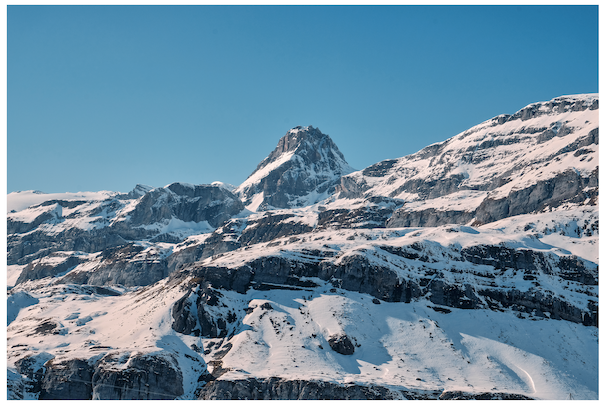
\includegraphics[width=\textwidth]{images/DSCF7228leukerbadsunset.png}}

\author{Dylan Lawless}
\title{Selected works}

\usepackage{fancyhdr}
\pagestyle{fancy}
\fancyhf{} % clear all fields
\fancyhead[L]{\small\nouppercase{\rightmark}}
\fancyhead[R]{\small\nouppercase{\leftmark}}
\fancyfoot[RO, LE] {\thepage}

% Redefine the plain page style for chapter page
\fancypagestyle{plain}{%
  \fancyhf{}%
\fancyhead[L]{\small\nouppercase{\rightmark}}
\fancyhead[R]{\small\nouppercase{\leftmark}}
\fancyfoot[RO, LE] {\thepage}
}